%Manuscript based on tutorial given by Fred J. Hickernell at MCQMC, August 14, 2016
%Requires graphics files
%  

\documentclass[graybox,footinfo]{svmult}

\smartqed
\usepackage{mathptmx}       % selects Times Roman as basic font
\usepackage{helvet}         % selects Helvetica as sans-serif font
\usepackage{courier}        % selects Courier as typewriter font
\usepackage{type1cm}        % activate if the above 3 fonts are
% not available on your system
\usepackage{graphicx}       % standard LaTeX graphics tool
% when including figure files

\usepackage{array,colortbl}
\usepackage{amsmath,amsfonts,amssymb,bm} % no amsthm, Springer defines Theorem, 
%Lemma, etc themselves
%\usepackage[mathx]{mathabx}
\DeclareFontFamily{U}{mathx}{\hyphenchar\font45}
\DeclareFontShape{U}{mathx}{m}{n}{
	<5> <6> <7> <8> <9> <10>
	<10.95> <12> <14.4> <17.28> <20.74> <24.88>
	mathx10
}{}
\DeclareSymbolFont{mathx}{U}{mathx}{m}{n}
\DeclareFontSubstitution{U}{mathx}{m}{n}
\DeclareMathAccent{\widecheck}      {0}{mathx}{"71}



% Note that Springer defines the following already:
%
% \D upright d for differential d
% \I upright i for imaginary unit
% \E upright e for exponential function
% \tens depicts tensors as sans serif upright
% \vec depicts vectors as boldface characters instead of the arrow accent
%
% Additionally we throw in the following common used macro's:
%%  This file will be included when we compile the final book. You can
%%  make use of the commonly used packages and commonly defined macros
%%  from here.
%%
%%  PLEASE DO NOT CHANGE THIS FILE.
%%  PLEASE DO NOT REDFINE ANY OF THE MACROS.
%%
%%  For convenience you may wish to define your own macros in your main
%%  tex file while preparing the manuscript. However, before submitting
%%  your final file for the accepted manuscript, we will ask you to replace
%%  your macros with the full commands.
%%

\renewcommand{\email}[1]{\emailname: #1} % change the email address font style

\usepackage{mathptmx}       % selects Times Roman as basic font
\usepackage{helvet}         % selects Helvetica as sans-serif font
\usepackage{courier}        % selects Courier as typewriter font
%\usepackage{type1cm}        % activate if the above 3 fonts are
%                            % not available on your system

\usepackage{makeidx}         % allows index generation
\usepackage{graphicx}        % standard LaTeX graphics tool
                             % when including figure files
%\usepackage{multicol}        % used for the two-column index
\usepackage[bottom]{footmisc}% places footnotes at page bottom

\usepackage{latexsym}
\usepackage{amsmath}
\usepackage{amsfonts}
\usepackage{amssymb}
\usepackage{bm}

\usepackage{url}
\usepackage{algorithm}
\usepackage{algorithmic}
\usepackage[misc,geometry]{ifsym}

% Springer provides the following environments:
%   case, conjecture, corollary, definition, example, exercise, lemma,
%   note, problem, property, proposition, question, remark, solution, theorem
%   claim, proof
\renewenvironment{proof}{\noindent{\itshape Proof.}}{\smartqed\qed}

% We add two more environments:   assumption, algo
\spdefaulttheorem{assumption}{Assumption}{\upshape \bfseries}{\itshape}
\spdefaulttheorem{algo}{Algorithm}{\upshape \bfseries}{\itshape}
% Note there is also the 'algorithm' environment from the algorithm package
% which is a floating environment



% Springer defines the following commands in math mode:
%   \D upright d for differential d
%   \I upright i for imaginary unit
%   \E upright e for exponential function
%   \tens depicts tensors as sans serif upright
%   \vec depicts vectors as boldface characters instead of the arrow accent


% We add the following commonly used macros:

% vectors as boldsymbols:
\newcommand{\bsa}{{\boldsymbol{a}}}
\newcommand{\bsb}{{\boldsymbol{b}}}
\newcommand{\bsc}{{\boldsymbol{c}}}
\newcommand{\bsd}{{\boldsymbol{d}}}
\newcommand{\bse}{{\boldsymbol{e}}}
\newcommand{\bsf}{{\boldsymbol{f}}}
\newcommand{\bsg}{{\boldsymbol{g}}}
\newcommand{\bsh}{{\boldsymbol{h}}}
\newcommand{\bsi}{{\boldsymbol{i}}}
\newcommand{\bsj}{{\boldsymbol{j}}}
\newcommand{\bsk}{{\boldsymbol{k}}}
\newcommand{\bsl}{{\boldsymbol{l}}}
\newcommand{\bsm}{{\boldsymbol{m}}}
\newcommand{\bsn}{{\boldsymbol{n}}}
\newcommand{\bso}{{\boldsymbol{o}}}
\newcommand{\bsp}{{\boldsymbol{p}}}
\newcommand{\bsq}{{\boldsymbol{q}}}
\newcommand{\bsr}{{\boldsymbol{r}}}
\newcommand{\bss}{{\boldsymbol{s}}}
\newcommand{\bst}{{\boldsymbol{t}}}
\newcommand{\bsu}{{\boldsymbol{u}}}
\newcommand{\bsv}{{\boldsymbol{v}}}
\newcommand{\bsw}{{\boldsymbol{w}}}
\newcommand{\bsx}{{\boldsymbol{x}}}
\newcommand{\bsy}{{\boldsymbol{y}}}
\newcommand{\bsz}{{\boldsymbol{z}}}
\newcommand{\bsA}{{\boldsymbol{A}}}
\newcommand{\bsB}{{\boldsymbol{B}}}
\newcommand{\bsC}{{\boldsymbol{C}}}
\newcommand{\bsD}{{\boldsymbol{D}}}
\newcommand{\bsE}{{\boldsymbol{E}}}
\newcommand{\bsF}{{\boldsymbol{F}}}
\newcommand{\bsG}{{\boldsymbol{G}}}
\newcommand{\bsH}{{\boldsymbol{H}}}
\newcommand{\bsI}{{\boldsymbol{I}}}
\newcommand{\bsJ}{{\boldsymbol{J}}}
\newcommand{\bsK}{{\boldsymbol{K}}}
\newcommand{\bsL}{{\boldsymbol{L}}}
\newcommand{\bsM}{{\boldsymbol{M}}}
\newcommand{\bsN}{{\boldsymbol{N}}}
\newcommand{\bsO}{{\boldsymbol{O}}}
\newcommand{\bsP}{{\boldsymbol{P}}}
\newcommand{\bsQ}{{\boldsymbol{Q}}}
\newcommand{\bsR}{{\boldsymbol{R}}}
\newcommand{\bsS}{{\boldsymbol{S}}}
\newcommand{\bsT}{{\boldsymbol{T}}}
\newcommand{\bsU}{{\boldsymbol{U}}}
\newcommand{\bsV}{{\boldsymbol{V}}}
\newcommand{\bsW}{{\boldsymbol{W}}}
\newcommand{\bsX}{{\boldsymbol{X}}}
\newcommand{\bsY}{{\boldsymbol{Y}}}
\newcommand{\bsZ}{{\boldsymbol{Z}}}
% other commonly used boldsymbols:
\newcommand{\bsell}{{\boldsymbol{\ell}}}
\newcommand{\bszero}{{\boldsymbol{0}}} % vector of zeros
\newcommand{\bsone}{{\boldsymbol{1}}}  % vector of ones
% boldsymbol greeks:
\newcommand{\bsalpha}{{\boldsymbol{\alpha}}}
\newcommand{\bsbeta}{{\boldsymbol{\beta}}}
\newcommand{\bsgamma}{{\boldsymbol{\gamma}}}
\newcommand{\bsdelta}{{\boldsymbol{\delta}}}
\newcommand{\bsepsilon}{{\boldsymbol{\epsilon}}}
\newcommand{\bsvarepsilon}{{\boldsymbol{\varepsilon}}}
\newcommand{\bszeta}{{\boldsymbol{\zeta}}}
\newcommand{\bseta}{{\boldsymbol{\eta}}}
\newcommand{\bstheta}{{\boldsymbol{\theta}}}
\newcommand{\bsvartheta}{{\boldsymbol{\vartheta}}}
\newcommand{\bskappa}{{\boldsymbol{\kappa}}}
\newcommand{\bslambda}{{\boldsymbol{\lambda}}}
\newcommand{\bsmu}{{\boldsymbol{\mu}}}
\newcommand{\bsnu}{{\boldsymbol{\nu}}}
\newcommand{\bsxi}{{\boldsymbol{\xi}}}
\newcommand{\bspi}{{\boldsymbol{\pi}}}
\newcommand{\bsvarpi}{{\boldsymbol{\varpi}}}
\newcommand{\bsrho}{{\boldsymbol{\rho}}}
\newcommand{\bsvarrho}{{\boldsymbol{\varrho}}}
\newcommand{\bssigma}{{\boldsymbol{\sigma}}}
\newcommand{\bsvarsigma}{{\boldsymbol{\varsigma}}}
\newcommand{\bstau}{{\boldsymbol{\tau}}}
\newcommand{\bsupsilon}{{\boldsymbol{\upsilon}}}
\newcommand{\bsphi}{{\boldsymbol{\phi}}}
\newcommand{\bsvarphi}{{\boldsymbol{\varphi}}}
\newcommand{\bschi}{{\boldsymbol{\chi}}}
\newcommand{\bspsi}{{\boldsymbol{\psi}}}
\newcommand{\bsomega}{{\boldsymbol{\omega}}}
\newcommand{\bsGamma}{{\boldsymbol{\Gamma}}}
\newcommand{\bsDelta}{{\boldsymbol{\Delta}}}
\newcommand{\bsTheta}{{\boldsymbol{\Theta}}}
\newcommand{\bsLambda}{{\boldsymbol{\Lambda}}}
\newcommand{\bsXi}{{\boldsymbol{\Xi}}}
\newcommand{\bsPi}{{\boldsymbol{\Pi}}}
\newcommand{\bsSigma}{{\boldsymbol{\Sigma}}}
\newcommand{\bsUpsilon}{{\boldsymbol{\Upsilon}}}
\newcommand{\bsPhi}{{\boldsymbol{\Phi}}}
\newcommand{\bsPsi}{{\boldsymbol{\Psi}}}
\newcommand{\bsOmega}{{\boldsymbol{\Omega}}}

% Roman fonts:
\newcommand{\rma}{{\mathrm{a}}}
\newcommand{\rmb}{{\mathrm{b}}}
\newcommand{\rmc}{{\mathrm{c}}}
\newcommand{\rmd}{{\mathrm{d}}}
\newcommand{\rme}{{\mathrm{e}}}
\newcommand{\rmf}{{\mathrm{f}}}
\newcommand{\rmg}{{\mathrm{g}}}
\newcommand{\rmh}{{\mathrm{h}}}
\newcommand{\rmi}{{\mathrm{i}}}
\newcommand{\rmj}{{\mathrm{j}}}
\newcommand{\rmk}{{\mathrm{k}}}
\newcommand{\rml}{{\mathrm{l}}}
\newcommand{\rmm}{{\mathrm{m}}}
\newcommand{\rmn}{{\mathrm{n}}}
\newcommand{\rmo}{{\mathrm{o}}}
\newcommand{\rmp}{{\mathrm{p}}}
\newcommand{\rmq}{{\mathrm{q}}}
\newcommand{\rmr}{{\mathrm{r}}}
\newcommand{\rms}{{\mathrm{s}}}
\newcommand{\rmt}{{\mathrm{t}}}
\newcommand{\rmu}{{\mathrm{u}}}
\newcommand{\rmv}{{\mathrm{v}}}
\newcommand{\rmw}{{\mathrm{w}}}
\newcommand{\rmx}{{\mathrm{x}}}
\newcommand{\rmy}{{\mathrm{y}}}
\newcommand{\rmz}{{\mathrm{z}}}
\newcommand{\rmA}{{\mathrm{A}}}
\newcommand{\rmB}{{\mathrm{B}}}
\newcommand{\rmC}{{\mathrm{C}}}
\newcommand{\rmD}{{\mathrm{D}}}
\newcommand{\rmE}{{\mathrm{E}}}
\newcommand{\rmF}{{\mathrm{F}}}
\newcommand{\rmG}{{\mathrm{G}}}
\newcommand{\rmH}{{\mathrm{H}}}
\newcommand{\rmI}{{\mathrm{I}}}
\newcommand{\rmJ}{{\mathrm{J}}}
\newcommand{\rmK}{{\mathrm{K}}}
\newcommand{\rmL}{{\mathrm{L}}}
\newcommand{\rmM}{{\mathrm{M}}}
\newcommand{\rmN}{{\mathrm{N}}}
\newcommand{\rmO}{{\mathrm{O}}}
\newcommand{\rmP}{{\mathrm{P}}}
\newcommand{\rmQ}{{\mathrm{Q}}}
\newcommand{\rmR}{{\mathrm{R}}}
\newcommand{\rmS}{{\mathrm{S}}}
\newcommand{\rmT}{{\mathrm{T}}}
\newcommand{\rmU}{{\mathrm{U}}}
\newcommand{\rmV}{{\mathrm{V}}}
\newcommand{\rmW}{{\mathrm{W}}}
\newcommand{\rmX}{{\mathrm{X}}}
\newcommand{\rmY}{{\mathrm{Y}}}
\newcommand{\rmZ}{{\mathrm{Z}}}
% also commonly defined
\newcommand{\rd}{{\mathrm{d}}}
\newcommand{\ri}{{\mathrm{i}}}

% blackboards:
\newcommand{\bbA}{{\mathbb{A}}}
\newcommand{\bbB}{{\mathbb{B}}}
\newcommand{\bbC}{{\mathbb{C}}}
\newcommand{\bbD}{{\mathbb{D}}}
\newcommand{\bbE}{{\mathbb{E}}}
\newcommand{\bbF}{{\mathbb{F}}}
\newcommand{\bbG}{{\mathbb{G}}}
\newcommand{\bbH}{{\mathbb{H}}}
\newcommand{\bbI}{{\mathbb{I}}}
\newcommand{\bbJ}{{\mathbb{J}}}
\newcommand{\bbK}{{\mathbb{K}}}
\newcommand{\bbL}{{\mathbb{L}}}
\newcommand{\bbM}{{\mathbb{M}}}
\newcommand{\bbN}{{\mathbb{N}}}
\newcommand{\bbO}{{\mathbb{O}}}
\newcommand{\bbP}{{\mathbb{P}}}
\newcommand{\bbQ}{{\mathbb{Q}}}
\newcommand{\bbR}{{\mathbb{R}}}
\newcommand{\bbS}{{\mathbb{S}}}
\newcommand{\bbT}{{\mathbb{T}}}
\newcommand{\bbU}{{\mathbb{U}}}
\newcommand{\bbV}{{\mathbb{V}}}
\newcommand{\bbW}{{\mathbb{W}}}
\newcommand{\bbX}{{\mathbb{X}}}
\newcommand{\bbY}{{\mathbb{Y}}}
\newcommand{\bbZ}{{\mathbb{Z}}}
% commonly used shortcuts:
\newcommand{\C}{{\mathbb{C}}} % complex numbers
\newcommand{\F}{{\mathbb{F}}} % field, finite field
\newcommand{\N}{{\mathbb{N}}} % natural numbers {1, 2, ...}
\newcommand{\Q}{{\mathbb{Q}}} % rationals
\newcommand{\R}{{\mathbb{R}}} % reals
\newcommand{\Z}{{\mathbb{Z}}} % integers
% more commonly used shortcuts:
\newcommand{\CC}{{\mathbb{C}}} % complex numbers
\newcommand{\FF}{{\mathbb{F}}} % field, finite field
\newcommand{\NN}{{\mathbb{N}}} % natural numbers {1, 2, ...}
\newcommand{\QQ}{{\mathbb{Q}}} % rationals
\newcommand{\RR}{{\mathbb{R}}} % reals
\newcommand{\ZZ}{{\mathbb{Z}}} % integers
% more commonly used shortcuts:
\newcommand{\EE}{{\mathbb{E}}}
\newcommand{\PP}{{\mathbb{P}}}
\newcommand{\TT}{{\mathbb{T}}}
\newcommand{\VV}{{\mathbb{V}}}
% and even more commonly used shortcuts:
\newcommand{\Complex}{{\mathbb{C}}}
\newcommand{\Integer}{{\mathbb{Z}}}
\newcommand{\Natural}{{\mathbb{N}}}
\newcommand{\Rational}{{\mathbb{Q}}}
\newcommand{\Real}{{\mathbb{R}}}
% indicator boldface 1:
\DeclareSymbolFont{bbold}{U}{bbold}{m}{n}
\DeclareSymbolFontAlphabet{\mathbbold}{bbold}
\newcommand{\ind}{{\mathbbold{1}}}
\newcommand{\bbone}{{\mathbbold{1}}}


% calligraphic letters:
\newcommand{\cala}{{\mathcal{a}}}
\newcommand{\calb}{{\mathcal{b}}}
\newcommand{\calc}{{\mathcal{c}}}
\newcommand{\cald}{{\mathcal{d}}}
\newcommand{\cale}{{\mathcal{e}}}
\newcommand{\calf}{{\mathcal{f}}}
\newcommand{\calg}{{\mathcal{g}}}
\newcommand{\calh}{{\mathcal{h}}}
\newcommand{\cali}{{\mathcal{i}}}
\newcommand{\calj}{{\mathcal{j}}}
\newcommand{\calk}{{\mathcal{k}}}
\newcommand{\call}{{\mathcal{l}}}
\newcommand{\calm}{{\mathcal{m}}}
\newcommand{\caln}{{\mathcal{n}}}
\newcommand{\calo}{{\mathcal{o}}}
\newcommand{\calp}{{\mathcal{p}}}
\newcommand{\calq}{{\mathcal{q}}}
\newcommand{\calr}{{\mathcal{r}}}
\newcommand{\cals}{{\mathcal{s}}}
\newcommand{\calt}{{\mathcal{t}}}
\newcommand{\calu}{{\mathcal{u}}}
\newcommand{\calv}{{\mathcal{v}}}
\newcommand{\calw}{{\mathcal{w}}}
\newcommand{\calx}{{\mathcal{x}}}
\newcommand{\caly}{{\mathcal{y}}}
\newcommand{\calz}{{\mathcal{z}}}
\newcommand{\calA}{{\mathcal{A}}}
\newcommand{\calB}{{\mathcal{B}}}
\newcommand{\calC}{{\mathcal{C}}}
\newcommand{\calD}{{\mathcal{D}}}
\newcommand{\calE}{{\mathcal{E}}}
\newcommand{\calF}{{\mathcal{F}}}
\newcommand{\calG}{{\mathcal{G}}}
\newcommand{\calH}{{\mathcal{H}}}
\newcommand{\calI}{{\mathcal{I}}}
\newcommand{\calJ}{{\mathcal{J}}}
\newcommand{\calK}{{\mathcal{K}}}
\newcommand{\calL}{{\mathcal{L}}}
\newcommand{\calM}{{\mathcal{M}}}
\newcommand{\calN}{{\mathcal{N}}}
\newcommand{\calO}{{\mathcal{O}}}
\newcommand{\calP}{{\mathcal{P}}}
\newcommand{\calQ}{{\mathcal{Q}}}
\newcommand{\calR}{{\mathcal{R}}}
\newcommand{\calS}{{\mathcal{S}}}
\newcommand{\calT}{{\mathcal{T}}}
\newcommand{\calU}{{\mathcal{U}}}
\newcommand{\calV}{{\mathcal{V}}}
\newcommand{\calW}{{\mathcal{W}}}
\newcommand{\calX}{{\mathcal{X}}}
\newcommand{\calY}{{\mathcal{Y}}}
\newcommand{\calZ}{{\mathcal{Z}}}

% Euler fraks:
\newcommand{\fraka}{{\mathfrak{a}}}
\newcommand{\frakb}{{\mathfrak{b}}}
\newcommand{\frakc}{{\mathfrak{c}}}
\newcommand{\frakd}{{\mathfrak{d}}}
\newcommand{\frake}{{\mathfrak{e}}}
\newcommand{\frakf}{{\mathfrak{f}}}
\newcommand{\frakg}{{\mathfrak{g}}}
\newcommand{\frakh}{{\mathfrak{h}}}
\newcommand{\fraki}{{\mathfrak{i}}}
\newcommand{\frakj}{{\mathfrak{j}}}
\newcommand{\frakk}{{\mathfrak{k}}}
\newcommand{\frakl}{{\mathfrak{l}}}
\newcommand{\frakm}{{\mathfrak{m}}}
\newcommand{\frakn}{{\mathfrak{n}}}
\newcommand{\frako}{{\mathfrak{o}}}
\newcommand{\frakp}{{\mathfrak{p}}}
\newcommand{\frakq}{{\mathfrak{q}}}
\newcommand{\frakr}{{\mathfrak{r}}}
\newcommand{\fraks}{{\mathfrak{s}}}
\newcommand{\frakt}{{\mathfrak{t}}}
\newcommand{\fraku}{{\mathfrak{u}}}
\newcommand{\frakv}{{\mathfrak{v}}}
\newcommand{\frakw}{{\mathfrak{w}}}
\newcommand{\frakx}{{\mathfrak{x}}}
\newcommand{\fraky}{{\mathfrak{y}}}
\newcommand{\frakz}{{\mathfrak{z}}}
\newcommand{\frakA}{{\mathfrak{A}}}
\newcommand{\frakB}{{\mathfrak{B}}}
\newcommand{\frakC}{{\mathfrak{C}}}
\newcommand{\frakD}{{\mathfrak{D}}}
\newcommand{\frakE}{{\mathfrak{E}}}
\newcommand{\frakF}{{\mathfrak{F}}}
\newcommand{\frakG}{{\mathfrak{G}}}
\newcommand{\frakH}{{\mathfrak{H}}}
\newcommand{\frakI}{{\mathfrak{I}}}
\newcommand{\frakJ}{{\mathfrak{J}}}
\newcommand{\frakK}{{\mathfrak{K}}}
\newcommand{\frakL}{{\mathfrak{L}}}
\newcommand{\frakM}{{\mathfrak{M}}}
\newcommand{\frakN}{{\mathfrak{N}}}
\newcommand{\frakO}{{\mathfrak{O}}}
\newcommand{\frakP}{{\mathfrak{P}}}
\newcommand{\frakQ}{{\mathfrak{Q}}}
\newcommand{\frakR}{{\mathfrak{R}}}
\newcommand{\frakS}{{\mathfrak{S}}}
\newcommand{\frakT}{{\mathfrak{T}}}
\newcommand{\frakU}{{\mathfrak{U}}}
\newcommand{\frakV}{{\mathfrak{V}}}
\newcommand{\frakW}{{\mathfrak{W}}}
\newcommand{\frakX}{{\mathfrak{X}}}
\newcommand{\frakY}{{\mathfrak{Y}}}
\newcommand{\frakZ}{{\mathfrak{Z}}}
% sets as Euler fraks:
\newcommand{\seta}{{\mathfrak{a}}}
\newcommand{\setb}{{\mathfrak{b}}}
\newcommand{\setc}{{\mathfrak{c}}}
\newcommand{\setd}{{\mathfrak{d}}}
\newcommand{\sete}{{\mathfrak{e}}}
\newcommand{\setf}{{\mathfrak{f}}}
\newcommand{\setg}{{\mathfrak{g}}}
\newcommand{\seth}{{\mathfrak{h}}}
\newcommand{\seti}{{\mathfrak{i}}}
\newcommand{\setj}{{\mathfrak{j}}}
\newcommand{\setk}{{\mathfrak{k}}}
\newcommand{\setl}{{\mathfrak{l}}}
\newcommand{\setm}{{\mathfrak{m}}}
\newcommand{\setn}{{\mathfrak{n}}}
\newcommand{\seto}{{\mathfrak{o}}}
\newcommand{\setp}{{\mathfrak{p}}}
\newcommand{\setq}{{\mathfrak{q}}}
\newcommand{\setr}{{\mathfrak{r}}}
\newcommand{\sets}{{\mathfrak{s}}}
\newcommand{\sett}{{\mathfrak{t}}}
\newcommand{\setu}{{\mathfrak{u}}}
\newcommand{\setv}{{\mathfrak{v}}}
\newcommand{\setw}{{\mathfrak{w}}}
\newcommand{\setx}{{\mathfrak{x}}}
\newcommand{\sety}{{\mathfrak{y}}}
\newcommand{\setz}{{\mathfrak{z}}}
\newcommand{\setA}{{\mathfrak{A}}}
\newcommand{\setB}{{\mathfrak{B}}}
\newcommand{\setC}{{\mathfrak{C}}}
\newcommand{\setD}{{\mathfrak{D}}}
\newcommand{\setE}{{\mathfrak{E}}}
\newcommand{\setF}{{\mathfrak{F}}}
\newcommand{\setG}{{\mathfrak{G}}}
\newcommand{\setH}{{\mathfrak{H}}}
\newcommand{\setI}{{\mathfrak{I}}}
\newcommand{\setJ}{{\mathfrak{J}}}
\newcommand{\setK}{{\mathfrak{K}}}
\newcommand{\setL}{{\mathfrak{L}}}
\newcommand{\setM}{{\mathfrak{M}}}
\newcommand{\setN}{{\mathfrak{N}}}
\newcommand{\setO}{{\mathfrak{O}}}
\newcommand{\setP}{{\mathfrak{P}}}
\newcommand{\setQ}{{\mathfrak{Q}}}
\newcommand{\setR}{{\mathfrak{R}}}
\newcommand{\setS}{{\mathfrak{S}}}
\newcommand{\setT}{{\mathfrak{T}}}
\newcommand{\setU}{{\mathfrak{U}}}
\newcommand{\setV}{{\mathfrak{V}}}
\newcommand{\setW}{{\mathfrak{W}}}
\newcommand{\setX}{{\mathfrak{X}}}
\newcommand{\setY}{{\mathfrak{Y}}}
\newcommand{\setZ}{{\mathfrak{Z}}}

% other commonly defined commands:
\newcommand{\wal}{{\rm wal}}
\newcommand{\floor}[1]{\left\lfloor #1 \right\rfloor} % floor
\newcommand{\ceil}[1]{\left\lceil #1 \right\rceil}    % ceil
\DeclareMathOperator{\cov}{Cov}
\DeclareMathOperator{\var}{Var}
\providecommand{\argmin}{\operatorname*{argmin}}
\providecommand{\argmax}{\operatorname*{argmax}}


% Macros below are now inclded in macros.tex from MCQMC 2016 web site
% This spot formerly included macros that are now in macros.tex

% indicator boldface 1:
\DeclareSymbolFont{bbold}{U}{bbold}{m}{n}
\DeclareSymbolFontAlphabet{\mathbbold}{bbold}
%\newcommand{\ind}{\mathbbold{1}}


\usepackage{microtype} % good font tricks

\usepackage[colorlinks=true,linkcolor=black,citecolor=black,urlcolor=black]{hyperref}
\urlstyle{same}
\usepackage{bookmark}
\pdfstringdefDisableCommands{\def\and{, }}
\makeatletter % to avoid hyperref warnings:
\providecommand*{\toclevel@author}{999}
\providecommand*{\toclevel@title}{0}
\makeatother

%%%%%%%%%%%%%%%%%%%%%%%%%%%%%%%%%%%%%%%%%%%%%%%%%%%%%%%%%%%%%%%%%%%%%%%%%%%%%%%%%%%%%%%%%


%Fred's additions
%
\usepackage{xspace}
\DeclareMathOperator{\Cov}{cov}
\DeclareMathOperator{\algn}{CNF}
\DeclareMathOperator{\disc}{DSC}
\DeclareMathOperator{\Var}{VAR}
\DeclareMathOperator{\sign}{sign}
\DeclareMathOperator{\GP}{\cg\!\!\cp}

%%%%%%%%%%%%%%%%%%%%%%%%%%%%%%%%%%%%%%%%%%%%%%%%%%%%%%%%%%%%%%%%%%%%%%%%%%%%%%%%%%%%%%%%%
\begin{document}
	\newtheorem{FJHLesson}{Lesson}
\newcommand{\corr}{\mathrm{corr}}
\newcommand{\std}{\textup{std}}
\newcommand{\Dt}{\textup{D}}
\newcommand{\Rn}{\textup{R}}


\newcommand{\mC}{\mathsf{C}}
\newcommand{\Ex}{\mathbb{E}}
\newcommand{\Prob}{\mathbb{P}}
\newcommand{\cf}{\mathcal{F}}
\newcommand{\cl}{\mathcal{L}}
\newcommand{\cn}{\mathcal{N}}
\newcommand{\Order}{\mathcal{O}}
\newcommand{\cm}{\mathcal{M}}
\newcommand{\cg}{\mathcal{G}}
\newcommand{\cp}{\mathcal{P}}
\newcommand{\cu}{\mathcal{U}}
\newcommand{\cx}{\mathcal{X}}
\newcommand{\cy}{\mathcal{Y}}
\newcommand{\cz}{\mathcal{Z}}
\newcommand{\natm}{\N_{0,m}}
\newcommand{\cube}{[0,1)^d}
\newcommand{\hf}{\hat{f}}
\newcommand{\rf}{\mathring{f}}
\newcommand{\tf}{\tilde{f}}
\newcommand{\hg}{\hat{g}}
\newcommand{\hmu}{\widehat{\mu}}
\newcommand{\hI}{\hat{I}}
\newcommand{\tvk}{\tilde{\bsk}}
\newcommand{\hS}{\widehat{S}}
\newcommand{\tS}{\widetilde{S}}
\newcommand{\wcS}{\widecheck{S}}
\newcommand{\rnu}{\mathring{\nu}}
\newcommand{\tnu}{\widetilde{\nu}}
\newcommand{\hnu}{\widehat{\nu}}
\newcommand{\homega}{\widehat{\omega}}
\newcommand{\wcomega}{\mathring{\omega}}
\newcommand{\fC}{\mathfrak{C}}
\newcommand{\nodes}{\{\bsz_i\}_{i=0}^{\infty}}
\newcommand{\nodesn}{\{\bsz_i\}_{i=0}^{n-1}}
\newcommand{\norm}[1]{\ensuremath{\left \lVert #1 \right \rVert}} 
\newcommand{\snorm}[1]{\ensuremath{\left \lVert #1 \right \rVert}} 
\newcommand{\bignorm}[1]{\ensuremath{\bigl \lVert #1 \bigr \rVert}}
\newcommand{\Bignorm}[1]{\ensuremath{\Bigl \lVert #1 \Bigr \rVert}}
\newcommand{\abs}[1]{\ensuremath{\bigl \lvert #1 \bigr \rvert}}
\newcommand{\bigabs}[1]{\ensuremath{\bigl \lvert #1 \bigr \rvert}}
\newcommand{\Bigabs}[1]{\ensuremath{\Bigl \lvert #1 \Bigr \rvert}}
\newcommand{\biggabs}[1]{\ensuremath{\biggl \lvert #1 \biggr \rvert}}
\newcommand{\Biggabs}[1]{\ensuremath{\Biggl \lvert #1 \Biggr \rvert}}
\newcommand{\ip}[3][{}]{\ensuremath{\left \langle #2, #3 \right \rangle_{#1}}}
\newcommand{\err}{\textrm{err}}
\newcommand{\tbsone}{\tilde{\bsone}}
\newcommand{\tvarrho}{\tilde{\varrho}}
\newcommand{\rvarrho}{\mathring{\varrho}}
\newcommand{\tc}{\tilde{c}}
\newcommand{\tbsc}{\tilde{\bsc}}
\newcommand{\tbsy}{\tilde{\bsy}}
\newcommand{\tmC}{\widetilde{\mC}}
\newcommand{\tz}{\tilde{z}}
\newcommand{\tbsz}{\tilde{\bsz}}

\allowdisplaybreaks


\title*{Error Analysis of Quasi-Monte Carlo Methods}
\author{Fred J. Hickernell}
\institute{Fred J. Hickernell
\at Department of Applied Mathematics,  Illinois Institute of Technology, 10 W. 32$^{\text{nd}}$ Street, RE 208, Chicago, IL 60616, USA 
\email{hickernell@iit.edu}}
\maketitle

\abstract{.} 

\section{Introduction}
Monte Carlo methods are used to approximate multivariate integrals that cannot be evaluated analytically, i.e.,  integrals of the form
\begin{equation}
\mu = \int_{\cx} f(\bsx) \, \nu(\D \bsx), \label{INT} \tag{INT}
\end{equation}
where $f:\cx \to \R$ is a measurable function, $\cx$ is a measurable set, and $\nu$ is a \emph{probability} measure.  Here, $\mu$ is the mean of $f(\bsX)$, where the random variable $\bsX$ has probability measure $\nu$.  Monte Carlo methods approximate $\mu$ by a weighted average of values of $f$ at a finite number of data sites, $\bsx_1, \ldots, \bsx_n$:
\begin{equation} \label{AppxINT} \tag{MC}
\hmu = \sum_{i=1}^n f(\bsx_i) w_i = \int_{\cx} f(\bsx) \, \hnu(\D \bsx), \qquad \sum_{i=1}^n  w_i = \hnu(\cx) = 1.
\end{equation}
The sampling measure, $\hnu$, assigns a weight $w_i$ to the function value at the $i^{\text{th}}$ data site, and may be written as $\hnu = \sum_{i=1}^n w_i \delta_{\bsx_i}$, where the $\delta_{\bst}$ denotes a Dirac measure concentrated at the point $\bst$.  For now our interpretation of ``Monte Carlo'' is quite broad---the data sites and the weights may be deterministic or random.  Later, we impose further constraints.

This tutorial describes how to characterize and analyze the error, $\mu - \hmu$.  Specifically, we ask
\emph{
\begin{list}{}{\setlength\leftmargin{7ex}\setlength\labelwidth{5ex}}
\item[Q1.] How do good sampling schemes, $\hnu$, make the error, $\mu - \hmu$, smaller?
\item[Q2.] How can the error be decreased by re-casting the problem, say with a different $f$ or $\nu$?
\item[Q3.] How many samples, $n$, are required to meet a specified error tolerance?
\end{list}}
\noindent The aim is to summarize some known---but perhaps not widely 
known---results.  We introduce and illustrate these results by examples.

\section{Big Data Survey} \label{FJH:sec:sleep} 
Did you get enough sleep last night?  Did you get more sleep than the average person?  
How much sleep did the average person get? The answer to this last question is simply 
$\mu = N^{-1} \sum_{j=1}^N f(j)$, where $f(j)$ denotes the hours of sleep of individual 
$j$ in a population of $N$ individuals.  For a large population, such as the adult 
population of the United States, collecting the data is difficult. So you might resort to a 
web survey, where you receive responses from individuals $x_1, \ldots, x_n$.  The error of 
your sample mean, $\widehat{\mu} = n^{-1} \sum_{i=1}^n f(x_i)$, may be expressed as a 
product of three quantities:
\begin{align}
\nonumber
\mu - \widehat{\mu} 
&= \frac{1}N \sum_{j=1}^N f(j) -  \frac 1n \sum_{i=1}^n f(x_i)  \\
\nonumber
&= - \frac{1}N \sum_{j=1}^N \bigl[ f(j) - \mu \bigr]\left ( \frac Nn \bbone_{\{x_i\}_{i=1}^n}(j) 
- 1 \right) \\
& = \underbrace{-\corr(f, \bbone_{\{x_i\}_{i=1}^n})}_{\algn^\Dt(f,\nu - \hnu)} \,
\underbrace{\sqrt{\frac{1 - n/N}{n/N}}}_{\disc^\Dt(\nu - \hnu)} \, 
\underbrace{\std(f)}_{\Var^\Dt(f)}, 
\label{FJH:eq:surveydettrio}
\end{align}
where the population covariance of two functions $f$ and $g$, with respective 
population means $\mu(f)$ and $\mu(g)$, is defined as 
\begin{equation*}
\Cov(f,g) : = \frac 1N \sum_{j=1} [f(j) - \mu(f)] [g(j) - \mu(g)], \qquad 
\std(f) : = \sqrt{\Cov(f,f)},
\end{equation*}
and direct calculation yields
\begin{equation*}
\std\left(\frac Nn \bbone_{\{x_i\}_{i=1}^n}\right) = \sqrt{\frac{1 - n/N}{n/N}}.
\end{equation*}

The expression of the error as a product of three quantities in 
\eqref{FJH:eq:surveydettrio} is an case of the \emph{trio identity}, introduced by Meng 
\cite{Men16a}.  In this example the integral, $\mu$, corresponds to a sum, 
and the probability measure $\nu$ is the uniform measure over the sample space $\{1, 
\ldots, N\}$.  The sampling measure corresponding to the web survey is $\hnu = 
n^{-1} \sum_{i=1}^n \delta_{x_i}$.  The three terms that comprise the trio identity have the 
following meanings:
\begin{description}
	\item[$\Var(f)$:] measures the \emph{variation} of the integrand from a typical value. 
	In 	this case, $\Var(f)$ corresponds to the standard deviation of $f$ and the typical 
	value	is the mean of $f$. The variation is positively homogeneous, i.e., $\Var(cf)  = 
	\abs{c} \Var(f)$.  The variation is \emph{not} the variance.
	\item [$\disc(\nu - \hnu)$:] measures the \emph{discrepancy} of the sampling 
	measure 
	from the probability measure that defines the integral.  In this case, the discrepancy 
	depends only on the sample fraction, $n/N$.
	\item [$\algn(f,\nu - \hnu)$:] measures the \emph{confounding} between the 
	integrand and the difference between the measure defining the integral and the 
	sampling measure.  In this case the confounding lies between plus and minus one.
\end{description}
The superscript $\Dt$ in \eqref{FJH:eq:surveydettrio} denotes a \emph{deterministic} 
version of the trio identity, which is defined in general in ???  Other versions of the trio 
identity will be introduced later.

For the web survey example one might expect $\Var(f)$ to be one or two hours or so.  It 
is inherent quality of what we are measuring and is not affected by our sampling 
scheme.  The discrepancy in this example will be quite large unless our survey includes a 
significant proportion of the population.  One might hope to make  the confounding 
small.  This will happen if the set of individuals who complete the survey 
is only weakly correlated with the number of hours of sleep.  Unfortunately, those who  
complete web surveys might tend to be those who are not sleeping as much as the 
population average.  It is difficult to estimate how small the confounding might be.  

An alternative to the web survey is a simple random sample.  In this 
case, we may use a 
\emph{randomized} version of the trio identity, which is defined in general in ???.  Starting 
from \eqref{FJH:eq:surveydettrio}, the 
error of a sleep survey using a simple random sample without replacement is
\begin{align}
\nonumber
\mu - \widehat{\mu} 
& = -\corr(f, \bbone_{\{x_i\}_{i=1}^n}) \,
\sqrt{\frac{1 - n/N}{n/N}} \, 
\std(f) \\
& = \underbrace{\frac{- \corr\bigl(f, \bbone_{\{x_i\}_{i=1}^n}\bigr)}
{\std_{\hnu} \bigl( \corr\bigl(f, \bbone_{\{x_i\}_{i=1}^n}\bigr)\bigr)}}_{\algn^\Rn(f,\nu - \hnu)} 
\, 
\underbrace{\sqrt{\frac{1-n/N}{n(1-1/N)}}}_{\disc^\Rn(\nu - \hnu)} \, 
\underbrace{\std(f)}_{\Var^\Dt(f)},
\label{FJH:eq:surveyrndtrio}
\end{align}
where $\std_{\hnu}$ means standard deviation with respect to the random sampling 
scheme, and direct calculation yields
\begin{equation*}
\std_{\hnu} \bigl( \corr\bigl(f, \bbone_{\{x_i\}_{i=1}^n}\bigr)\bigr) = \sqrt{\frac{1}{N-1}}.
\end{equation*}

For the randomized trio identity, the confounding may now be greater than one in 
magnitude.  However, it confounding does have zero mean and 
standard deviation one.  This means that with probability $1-\alpha$, the magnitude of 
the confounding will be no greater than $1/\sqrt{\alpha}$ by Chebyshev's inequality. The 
sampling scheme generated by a web survey is in the sample space of the simple 
random survey, which is all possible choices of $n$ out of $N$ individuals.  Unless the 
web survey has a value of $\corr(f, \bbone_{\{x_i\}_{i=1}^n})$ 
on the order of $\Order(1/\sqrt{N})$, then it is one of the ``unfortunate minority'' of 
sampling schemes.

While the randomized confounding may be larger than in the deterministic case, 
the randomized discrepancy is $\Order(1/\sqrt{N})$ than in the 
deterministic case.  Comparing \eqref{FJH:eq:surveyrndtrio} with 
\eqref{FJH:eq:surveydettrio}, we conclude that for a large population a web survey with 
$n_{\textup{web}}$ samples is equivalent to a simple random survey with 
\[
n_{\textup{SRS}} \approx \frac{n_{\textup{web}}/N}{\corr^2\Bigl(f, 
\bbone_{\{x_i\}_{i=1}^{n_{\textup{web}}}}\Bigr)(1-n_{\textup{web}}/N)}
\]
samples.  For example, an exceedingly successful web survey with $n_{\textup{web}} = 
1$ million distinct responses from a population of $N = 250$ million 
(approximately the US adult population) with a correlation as small as $0.05$ is about as 
valuable as $n_{\textup{SRS}} = 1.6$ simple random samples.

This example cautions against becoming too enthralled with big data. Unless the sample 
fraction is close to one or the correlation between 
your sampling scheme and what you are measuring can be made tiny, a large quantity of 
data may give a worse answer than a small quantity of carefully collected data.

\begin{FJHLesson}
	Systematic sampling may yield a much smaller error than haphazard sampling.
\end{FJHLesson}

\section{The Deterministic Trio Identity for Cubature Error}
The two versions of the trio identity introduced by example in the previous section may 
be defined in generality. We begin with the deterministic version.  

The integrand is 
assumed to lie in some Banach space of 
functions, $(\cf,\norm{\cdot}_{\cf})$, where function evaluation at any point  in the 
domain,  $\cx$, is a 
bounded, linear functional.  This means that $\sup_{f \in \cf} \abs{f(\bst)}/\norm{f}_{\cf} < 
\infty$ for all $\bst \in \cx$ and that $\int_{\cx} f(\bsx) \, \delta_{\bst}(\D\bsx) =f(\bst)$ 
for all $f \in \cf, \ \bst \in \cx$, where $\delta_{\bst}$ denotes the Dirac measure 
concentrated at $\bst$.  Let $L :\cf \to \R$ be some bounded 
linear functional.  If $L(f) \ne 0$ for any $f$, then $\cf$ is assumed to contain all 
constant functions.  The deterministic discrepancy is defined as 
\begin{equation}  \label{FJH:eq:detvardef}
\Var^{\Dt}(f) := \norm{f- L(f)}_{\cf} \qquad \forall f \in \cf.
\end{equation} 

Let $\cm$ denote the vector space of signed measures for which integrands in $\cf$ 
have finite integrals:
\begin{equation*}
\cm : = \biggl \{\text{signed measures } \eta : \int_{\cx} f(\bsx) \, \eta(\D\bsx) < \infty \ \ 
\forall f \in \cf \biggr \}.
\end{equation*}
It is assumed that $\nu \in \cm$ so that our integral of interest is defined.  Since function 
evaluation is bounded, $\cm$ includes the Dirac measures and also any 
sampling measure, $\hnu = \sum_{i=1}^n w_i \delta_{\bsx_i}$.  Define the subspace  
\begin{equation} \label{FJH:eq:Mperpdef}
\cm_\bot : = \left \{\eta \in \cm :  \int_{\cx} L(f) \, \eta(\D\bsx) = 0  \ \forall f \in \cf
\right\}.
\end{equation} 
A semi-norm on $\cm_\bot$ is induced by the norm on $\cf$, which provides the 
definition of discrepancy:
\begin{equation} \label{FJH:eq:detdiscdef}
\snorm{\eta}_{\cm_\bot}  : =\sup_{f \in \cf : f \ne 0} \frac{\displaystyle \biggabs{\int_{\cx} 
f(\bsx) \, \eta(\D \bsx)}}{\norm{f}_{\cf}}, \qquad \disc^\Dt(\nu - \hnu) : = \norm{\nu - 
\hnu}_{\cm_\bot}.
\end{equation}

Finally, define the confounding as 
	\begin{equation} \label{FJH:eq:detconfdef}
\algn^\Dt(f,\nu - \hnu): =  \begin{cases} \displaystyle 
\frac{\displaystyle\int_{\cx} f(\bsx) \, (\nu - \hnu)(\D 
	\bsx)}{\Var^\Dt(f)\disc^\Dt(\nu - \hnu)},  & 
\Var^\Dt(f)\disc^\Dt(\nu - \hnu) \ne 0, \\[2ex]
0, & \text{otherwise}.
\end{cases}
\end{equation}
The above definitions allow us to establish the deterministic trio identity for cubature 
error.

\begin{theorem}[Deterministic Trio Error Identity]  For the spaces of integrands and 
measures defined above, and for the above definitions of variation, discrepancy, and 
confounding, the following error identity holds for all $f \in \cf$ and $\nu - \hnu  \in 
\cm_\bot$: 
\begin{equation} \tag{DTRIO} \label{FJH:eq:dtrio}
\mu - \hmu  = \algn^\Dt(f,\nu - \hnu) \, \disc^\Dt(\nu - \hnu) \, \Var^{\Dt}(f).
\end{equation}
Moreover, $\abs{\algn(f,\nu - \hnu)} \le 1$. 
\end{theorem}
\begin{proof}  The proof of this identity follows directly from the definitions above, by 
noting that for all $f \in \cf$ and $\nu - \hnu  \in \cm_\bot$, the error can be written as a 
single integral via \eqref{INT} and \eqref{AppxINT}:
	\begin{equation} \label{FJH:eq:err_as_int}
	\mu - \hmu   =  \int_{\cx} f(\bsx) \, (\nu - \hnu)(\D \bsx).
	\end{equation}
	If $\Var^{\Dt}(f) = 0$, then $f = L(f)$, and the integral above vanishes due to the 
	definition of $\cm_{\bot}$.  If $\disc^\Dt(\nu - \hnu) = 0$, then the integral above 
	vanishes by \eqref{FJH:eq:detdiscdef}.  Thus, for $\Var^{\Dt}(f) \disc^\Dt(\nu - \hnu) = 
	0$ 
	the trio identity holds. If $\Var^{\Dt}(f) \disc^\Dt(\nu - \hnu) \ne 0$, then the trio 
	identity also holds by the definition of the confounding.
	
	Next, we analyze the magnitude of the confounding for $\Var^{\Dt}(f) \disc^\Dt(\nu - 
	\hnu) \ne 0$: 
	\begin{align*}
	\abs{\algn(f,\nu - \hnu)} & = 
		\frac{\biggl \lvert\displaystyle\int_{\cx} f(\bsx) \, (\nu - \hnu)(\D 
			\bsx) \biggr \rvert}{\Var^\Dt(f)\disc^\Dt(\nu - \hnu)} \quad \text{by 
			\eqref{FJH:eq:detconfdef}}\\
		& = \frac{\biggl \lvert\displaystyle\int_{\cx} [f(\bsx) - L(f)] \, (\nu - \hnu)(\D 
			\bsx) \biggr \rvert}{\norm{f-L(f)}_{\cf}\disc^\Dt(\nu - \hnu)} \quad \text{by 
			\eqref{FJH:eq:detvardef} and \eqref{FJH:eq:Mperpdef}} \\
		& \le 1 \quad \text{by \eqref{FJH:eq:detdiscdef}},
\end{align*}
since $\Var^{\Dt}(f) \ne 0$ and so $f - L(f) \ne 0$.
\end{proof}

Because the confounding has magnitude no greater than one, the deterministic trio 
identity may be converted into a deterministic error bound by 
ignoring the confounding:  $\abs{\mu - \hmu}  \le \disc^\Dt(\nu - \hnu) \, \Var^{\Dt}(f)$.  
Cubature error bounds of this form have a long history, dating back to the inequalities of 
Koksma \cite{Kok42} and Hlawka \cite{Hla61}. See also the monograph of Niederreiter 
\cite{Nie92}.  The confounding can be understood as the actual error divided by the 
absolute worst-case error.

For the big data sleep survey in Sec.\ \ref{FJH:sec:sleep}, $\cf$ is the space of all 
real-valued functions on $\cx := \{1, \ldots, N\}$ with scaled $\ell^2$ norm 
$\norm{f}_{\cf} 
:= N^{-1/2} \Bignorm{\bigl(f(j)\bigr)_{j=1}^N}_{\ell^2}$, and $L(f) := N^{-1}\sum_{j=1}^N f(j) 
= 
\mu $ is the population mean of $f$. It then follows that the variation of 
the integrand, $f$, is its standard deviation, as is seen in \eqref{FJH:eq:surveydettrio}.
The corresponding space of measures of interest is $\cm_\bot := \bigl \{ \sum_{i=1}^N u_j 
\delta_{j} : (u_1, \ldots, u_N) \in \R^N,\ u_1 + \cdots + u_N= 0 \bigr \}$, and its norm is 
$\bignorm{\sum_{i=1}^N u_i \delta_{i}}_{\cm_\bot} : = 
	\sqrt{N} \Bignorm{\bigl(u_i\bigr)_{i=1}^N}_{\ell^2}$.   The expressions for the 
	deterministic 
	discrepancy and confounding in \eqref{FJH:eq:surveydettrio} follow from these 
	choices.

When $\cf$ is a Hilbert space with reproducing kernel $K$, the discrepancy takes a 
simple, explicit form in terms of $K$.  The reproducing kernel is the unique function, $K: 
\cx \times \cx \to \R$ satisfying these two properties:
\begin{equation}
K(\cdot,\bst) \in \cf \quad \forall \bst \in \cx, \qquad f(\bst) = \ip[\cf]{K(\cdot,\bst)}{f} 
\quad \forall f \in \cf, \ \bst \in \cx.
\end{equation}
The Riesz Representation Theorem allows one to write the representer of cubature error 
as 
\begin{equation}
\eta_{\err}(\bst) = \ip[\cf]{K(\cdot,\bst)}{\eta_{\err}} = \int_{\cx} K(\bsx,\bst) \, (\nu - 
\hnu)(\D\bsx).
\end{equation}
Thus, 
\begin{equation}
\mu - \widehat{\mu} =  \ip[\cf]{\eta_{\err}}{f} = 
\underbrace{\frac{\ip[\cf]{\eta_{\err}}{f}}{\norm{f - 
L(f)}_{\cf} \norm{\eta_{\err}}_{\cf}} }_{\algn^\Dt(f,\nu - \hnu)}\, 
\underbrace{\norm{\eta_{\err}}_{\cf}}_{\disc^{\Dt}(\nu - \hnu)} \, 
\underbrace{\norm{f - L(f)}_{\cf}}_{\Var^\Dt(f)}
\end{equation}
provided that $\int_{\cx} L(f) \, (\nu - \hnu)(\D \bsx) = 0$.  The discrepancy  takes the 
form \cite{Hic99a}
\begin{align}
\nonumber
[\disc^{\Dt}(\nu - \hnu)]^2 & = \norm{\eta_{\err}}_{\cf}^2 = \ip[\cf]{\eta_{\err}}{\eta_{\err}} 
\\
\nonumber
& = \int_{\cx \times \cx} K(\bsx,\bst) \, (\nu - \hnu)(\D \bsx) \, (\nu - \hnu)(\D \bst) \\
\nonumber
& = \int_{\cx \times \cx} K(\bsx,\bst) \, \nu(\D \bsx) \, \nu (\D \bst)  \\
& \qquad \qquad - 2 \sum_{i=1}^n w_i 
\int_{\cx} K(\bsx,\bsx_i) \, \nu(\D \bsx)+ \sum_{i,j = 1}^n w_iw_jK(\bsx_i,\bsx_j).
\end{align}
The computational cost to evaluate the discrepancy is $\Order(n^2)$ times the cost of 
evaluating the reproducing kernel at a point. 

Note that in the reproducing kernel Hilbert space case, the confounding corresponds to 
the cosine of the angle between the integrand, $f$, and the representer of the error, 
$\eta_{\err}$.  This cosine is no greater than one in magnitude, as expected.

A particular example of this reproducing kernel Hilbert space setting corresponds to 
$\nu$ $v$ being the uniform probability measure on the $d$-dimensional unit cube, $\cx 
= 
[0,1]^d$, and the reproducing kernel defined by \cite{Hic97a}
\begin{equation} \label{FJH:eq:L2Kdef}
K(\bsx,\bst) =\prod_{k = 1}^d [2 - \max(x_k,t_k)],
\end{equation}
which is plotted in Fig.\ \ref{FJH:fig:L2ker}.  In this example, $L(f) = f(\bsone)$, and the 
variation is defined as
\begin{equation*}
\Var^\Dt(f)  = \norm{f-f(\bsone)}_\cf = \Bigl \lVert \bigl ( \norm{\partial^\fraku f}_{L^2}\bigr 
)_{\emptyset \subsetneq \fraku \subseteq 1:d} \Bigr \rVert_{\ell^2} , \qquad 
\partial^\fraku f : = \frac{\partial^{\lvert\fraku\rvert} f}{\partial \bsx_\fraku} \biggr 
\rvert_{\bsx_{\bar{\fraku}} = \bsone}.
\end{equation*}
Here $1\!:\!d : = \{1, \ldots, d\}$, $x_\fraku := (x_k)_{k \in \fraku}$, and $\bar{\fraku}$ 
denotes the complement of $\fraku$.  
The square discrepancy for the case where $w_i = 1/n$ is
\begin{align}
\nonumber
[\disc^\Dt(\nu - \hnu)]^2  &= \left(\frac 43\right)^d - \frac{2}n \sum_{i=1}^n \prod_{k=1}^d 
\left (\frac{3 - x_{ik}^2}{2} \right) + \frac{1}{n^2}\sum_{i,j=1}^n \prod_{k = 1}^d [2 - 
\max(x_{ik},x_{jk})] 
\\ &= \Bigl \lVert \bigl ( \norm{\nu([\bszero,\cdot_\fraku]) - 
	\hnu([\bszero,\cdot_\fraku])}_{L^2}\bigr )_{\emptyset \subsetneq \fraku \subseteq 1:d} 
	\Bigr 
	\rVert_{\ell^2}. \label{FJH:eq:L2disc}
\end{align}

This discrepancy has a geometric interpretation. Fig.\ \ref{FJH:fig:L2ker} displays the 
projections of some arbitrary 
data sites, $\bsx_{1,\fraku}, \ldots, \bsx_{n,\fraku}$, for $n=32$ and $\fraku = \{5,8\}$.  
Also 
shown is $\bsx_\fraku$, where $\bsx = (\ldots, 0.6, \ldots, 0.4, \ldots)$. The interval 
$[\bszero,\bsx_\fraku]$ has volume $0.24$ under the uniform measure, $\nu$, However, 
$[\bszero,\bsx_\fraku]$ only has 
volume $7/32 = 0.21875$ under the sampling measure, $\hnu$, corresponding to the 
proportion of data sites lying inside the interval $[\bszero,\bsx_\fraku]$. The difference is 
$0.02125$.  The average of this kind of difference, for all $\bsx \in [0,1]^d$ and for all 
$\emptyset \subsetneq \fraku 
\subseteq 1\!:\!d$ is what comprises the discrepancy above, which is called the 
$L^2$-discrepancy.

\begin{figure}
	\centering
	\includegraphics[height = 4cm]{ProgramsImages/L2Kernel.eps}\qquad
	\includegraphics[height = 4cm]{ProgramsImages/LocalDiscrep.eps}
	\caption{The left depicts the reproducing kernel in \eqref{FJH:eq:L2Kdef} for the 
	$L^2$-discrepancy 
	for $d=1$.  The right depicts the geometric interpretation of the discrepancy.
	\label{FJH:fig:L2ker}}
\end{figure}

If the data sites  $\bsx_{1}, \ldots, \bsx_{n}$ are chosen to be independent and identically 
distributed (IID) with probability measure $\nu$, and $w_1 = \cdots = w_n = 1/n$, then 
the mean square discrepancy for 
the reproducing Hilbert space case is
\begin{equation*}
[\disc^{\Dt}(\nu - \hnu)]^2  = \frac 1 n \left [ \int_{\cx} K(\bsx,\bsx) \, \nu(\D \bsx) - 
\int_{\cx \times \cx} K(\bsx,\bst) \, \nu(\D \bsx) \, \nu (\D \bst) \right ].
\end{equation*}
For the $L^2$ discrepancy in \eqref{FJH:eq:L2disc} this becomes 
\begin{equation} \label{FJH:eq:IIDL2disc}
[\disc^{\Dt}(\nu - \hnu)]^2  = \frac 1 n \left [ \left(\frac 32\right)^d - 
\left(\frac 43\right)^d \right ].
\end{equation}

In all versions of the trio identity, the discrepancy is the key term that should converge to 
zero as the sample size tends to infinity.  The variation is independent of the sample 
size, and the confounding may decrease, increase or oscillate with increasing $n$.  From 
the formulas above, the convergence of the discrepancy to zero for IID sampling as $n 
\to 
\infty$ is  $\Order(1/\sqrt{n})$, which is consistent with the expected convergence of the 
cubature error for IID Monte Carlo.  From \eqref{FJH:eq:IIDL2disc} we see that the 
value of the discrepancy may depend strongly on the dimension, $d$.  We return 
to this matter in Sec.\ ???

Quasi-Monte Carlo methods choose the data sites $\{\bsx_i\}_{i=1}^n$ to be dependent 
and more evenly spread than IID points.  For integration over $\cx = [0,1]^d$ with 
respect to the uniform measure, the data sites may be chosen to be
\begin{itemize} 
\item a digital net \cite{DicPil10a}, such as that proposed by Sobol' \cite{}, Faure \cite{}, 
Niederreiter \cite{} or Niederreiter and Xing \cite{}, or 
\item a node set of an integration lattice \cite{SloJoe94}.  
\end{itemize}
For details on the 
constructions of such sets, see the references above and Pierre L'Ecuyer's tutorial 
\cite{}.  The evenly spread data sites are often called \emph{low discrepancy} sets 
because the discrepancy in \eqref{FJH:eq:L2disc} and its relatives is 
$\Order(1/n^{1-\epsilon})$ as $n \to \infty$ for any positive $\varepsilon$.  Fig.\ 
\ref{FJH:fig:plotsdiffpts} displays examples of IID and low discrepancy points.

\begin{figure}
	\centering
	\includegraphics[height=5cm]{ProgramsImages/IIDPoints.eps} \quad
	\includegraphics[height=5cm]{ProgramsImages/ShiftedLatticePoints.eps} \\
	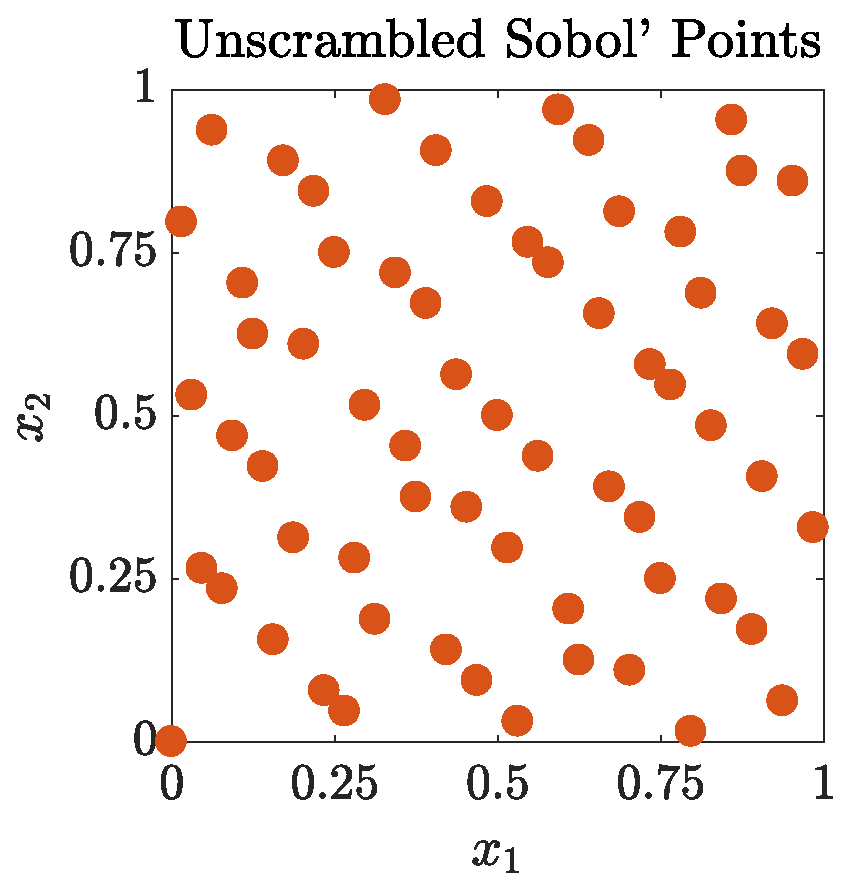
\includegraphics[height=5cm]{ProgramsImages/USobolPoints.eps} \quad
	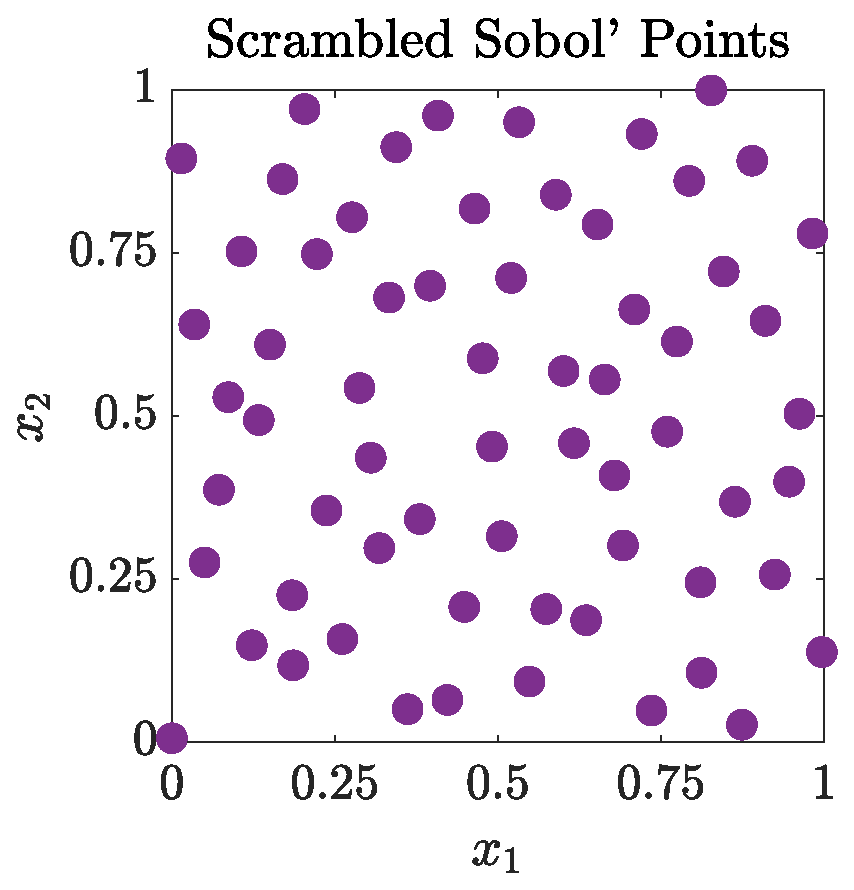
\includegraphics[height=5cm]{ProgramsImages/SSobolPoints.eps}
	\caption{An illustration of IID points and three examples of low discrepancy points 
	\label{FJH:fig:plotsdiffpts}}
\end{figure}



Graphs of discerpancy???

\section{The Randomized Trio Identity for Cubature Error}

\section{Multivariate Gaussian Probabilities}

When $\cx \ne [0,1]^d$ and/or $\nu$ is not the uniform 
measure, then one often resorts to transforming the integration variables or transforming 
the original points (see ??).


\


\begin{example}[Multivariate Probabilities] \label{MultivarProbA} If $g$ is the probability density function of some random variable $Y$ with sample space $\cy$, and $\cz \subset \cy$, then 
\[
\Prob(Y \in \cz) = \int_{\cz} g(\bsy) \, \D \bsy.
\]
This integral may be put in the form of \eqref{INT}---perhaps via a change of variables.  
For example (normal probability)
\end{example}

\begin{example}[Option Pricing]
\end{example}

\begin{example}[Sensitvity Analysis]
\end{example}



\section{The Trio Cubature Error Identity}
The \emph{trio identity}, first introduced by  \cite{Meng}, can describe various characterizations of the cubature error:
\begin{equation}
\mu - \hmu = \algn(f,\nu - \hnu) \disc(\nu - \hnu)  \Var(f). \label{trio}\tag{TRIO}
\end{equation}
This section derives various versions of this identity.  Here,
\begin{itemize}
\item $\algn(f,\nu - \hnu)$ measures the \emph{alignment} of the integrand with the difference between the measure defining the integral and the sampling measure,
\item $\disc(\eta)$ is the size of the measure $\eta$, so $\disc(\nu - \hnu)$ measures the \emph{discrepancy} of the sampling measure from the probability measure defining the integral, or equivalently,  and 
\item $\Var(f)$ measures the \emph{variation} of of the integrand from a constant value.
\end{itemize}
In general, we prefer these quantities to small, which keeps the cubature error small.  Better sampling schemes decrease the discrepancy.  A reformulation of the problem may yield an integrand with smaller variation.  The alignment is essentially scale invariant, while the discrepancy and variation are positively homogeneous.  For all $c_1, c_2, \in \R$,
\begin{gather*}
\algn(c_1f,c_2(\nu - \hnu)) =  \sign(c_1 c_2) \algn(f,\nu - \hnu) \\
\disc(c_2(\nu-\hnu))  = \abs{c_2} \disc(\nu-\hnu), \qquad  \Var(c_1f) =  \abs{c_1}\Var(f).
\end{gather*}

One may view the sampling scheme and integrand and as \emph{deterministic}.  
Alternatively, one may also consider \emph{randomized} sampling schemes and/or take a 
\emph{Bayesian} view of the integrand as a sample of a stochastic process.  All possible 
combinations lead to variations of \eqref{trio}.  Here we use more general concepts of 
the discrepancy and the variation than are common.  The goal is to unify the 
presentation of the error analysis.




The left side of the cubature error trio identity depends only on $f$, $\nu$, and $\hnu$, whereas the right side also depends on the space of integrands, $\cf$.  Changing $\cf$ generally changes all three terms in the right side of the trio identity---the variation, discrepancy, and cosine---because the definition of $\cm$ and its norm depends on $\cf$.  However, their product, which does not depend on $\cf$, remains the same.  Thus

\subsection{Reproducing Kernel Hilbert Spaces}
When $\cf$ is a Hilbert space with reproducing kernel $K$, the discrepancy takes a simple, explicit form in terms of $K$.  The reproducing kernel is the unique function, $K: \cx \times \cx \to \R$ satisfying these two properties:
\begin{equation}
K(\cdot,\bst) \in \cf \quad \forall \bst \in \cx, \qquad f(\bst) = \ip[\cf]{K(\cdot,\bst)}{f} \quad \forall f \in \cf, \ \bst \in \cx.
\end{equation}
The Riesz Representation Theorem allows one to write the representer of cubature error as 
\begin{equation}
\eta_{\err}(\bst) = \ip[\cf]{K(\cdot,\bst)}{\eta_{\err}} = \int_{\cx} K(\bsx,\bst) \, (\nu - \hnu)(\D\bsx).
\end{equation}
Thus, 

\subsection{The Koksma-Hlawka Error Bound Inequality}
The example above is an example o

\subsection{The Randomized Trio Error Identity}

\subsection{Bayesian Versions of the Trio Error Identity}

\subsection{Change of Variables}


\section{Minimizing the Discrepancy of the Sampling Scheme, $\norm{\nu - \hnu}_{\cm}$}

Tractability

\section{Minimizing the Variation of the Integrand, $\norm{f - L(f)}_{\cf}$}

\section{Minimizing the Cosine, $\algn(f - L(f),\nu - \hnu)$}

\section{Adaptive Cubature}
Via Bayesian approach

Via our approach

Various ideas
\begin{itemize}
\item series spaces
\item complexity bounds
\item tractability
\item multilevel methods
\item multivariate decomposition method, new Frances paper
\end{itemize}

\bibliographystyle{spmpsci}
\bibliography{FJH23,FJHown23}

\appendix
\section{Appendix}
\subsection{Gaussian Processes}
Suppose that $f:\cx \to \R$ is a Gaussian process with mean $m$ and covariance kernel $C(\cdot,\cdot)$, i.e., $f \sim \GP(m,C)$.  For fixed $\{\bsx_i\}_{i=1}^n$, the joint probability density function of $\bigl(f(\bsx_i)\bigr)_{i=1}^n$ is $\varrho$, defined as 
\begin{equation*}
\varrho (\bsy) = \frac{\exp\bigl(-\frac 12 (\bsy - m \bsone)^T \mC^{-1} (\bsy - m \bsone) \bigr)}{\sqrt{(2 \pi)^n \det(\mC)}}, \quad \bsy \in \R^n, \qquad \mC = \bigl(C(\bsx_i,\bsx_j)\bigr)_{i,j=1}^n.
\end{equation*}
Furthermore, the joint probability density function of $\bigl(\int_{\cx} f(\bsx) \, (\nu -\hnu)(\D \bsx), f(\bsx_1), \ldots, f(\bsx_n)\bigr)$ is $\tvarrho$, defined as 
\begin{align*}
\tvarrho (\tbsy) &= \frac{\exp\bigl(-\frac 12 (\tbsy - m \tbsone)^T \tmC^{-1} (\tbsy - m t\bsone) \bigr)}{\sqrt{(2 \pi)^{n+1} \det(\tmC)}}, \quad \tbsy = (y_i)_{i=0}^n \in \R^{n+1}, \\
 \tmC &= \begin{pmatrix} c_0 & \bsc^T \\ \bsc & \mC \end{pmatrix}, \qquad \tbsone = \bigl(1 - \bsone^T\bsw,  1, \ldots, 1 \bigr)^T, \\
 c_0 &= \int_{\cx^2} C(\bsx,\bst) \, (\nu -\hnu)(\D\bsx)(\nu -\hnu)(\D\bst) \\ 
 & = \int_{\cx^2} C(\bsx,\bst) \, \nu (\D\bsx)\nu(\D\bst) - 2 \sum_{i=1}^n w_i \int_{\cx} C(\bsx_i,\bsx) \, \nu (\D\bsx) +  \sum_{i,j=1}^n w_i w_j C(\bsx_i,\bsx_j)\\
 & = \tc_0 -2 \tbsc^T \bsw + \bsw^T \mC \bsw,\\
 & \qquad \qquad   \tc_0 = \int_{\cx^2} C(\bsx,\bst) \, \nu (\D\bsx)\nu(\D\bst), \qquad 
 \tbsc = \biggl( \int_{\cx} C(\bsx_i,\bsx) \, \nu (\D\bsx)\biggr)_{i=1}^n \\
 \bsc &= \biggl( \int_{\cx} C(\bsx,\bsx_i) \, (\nu -\hnu)(\D \bsx)\biggr)_{i=1}^n 
 =  \tbsc - \mC \bsw.
\end{align*}
Then the conditional probability density function of $\int_{\cx} f(\bsx) \,  (\nu -\hnu)(\D \bsx)$ given $\{f(\bsx_i )= y_i\}_{i=1}^n$ is $\rvarrho$, given by
\begin{equation*}
\rvarrho(y_0)  = \frac{\tvarrho(\tbsy)}{\varrho(\bsy)}  = \frac{\exp\bigl(-\frac 12 (\tbsy - m \tbsone)^T \tmC^{-1} (\tbsy - m \tbsone) + \frac 12 (\bsy - m \bsone)^T \mC^{-1} (\bsy - m \bsone)\bigr)}{\sqrt{2 \pi \det(\tmC)/\det(\mC)}}
\end{equation*}

To simplify the expression for $\rvarrho(y_0)$, we define
\[
\bsz = \mC^{-1} (\bsy - m \bsone), \qquad 
\begin{pmatrix} \tz_0 \\ \tbsz \end{pmatrix} = \tmC^{-1} (\tbsy - m \tbsone) 
= \begin{pmatrix} c_0 & \bsc^T \\ \bsc & \mC \end{pmatrix}^{-1} \begin{pmatrix} y_0 - m \\ \bsy - m \bsone \end{pmatrix}
\]
So,
\begin{gather*}
\begin{pmatrix} c_0 & \bsc^T \\ \bsc & \mC \end{pmatrix} \begin{pmatrix} \tz_0 \\ \tbsz \end{pmatrix} 
= \begin{pmatrix} y_0 - m(1 - \bsone^T\bsw) \\ \bsy - m \bsone \end{pmatrix} \\
\tbsz = \mC^{-1}[-\tz_0 \bsc + (\bsy - m \bsone )] \\
c_0 \tz_0 =y_0 - m(1 - \bsone^T\bsw)  - \bsc^T\tbsz =  y_0 - m(1 - \bsone^T\bsw)  - \bsc^T\mC^{-1}[-\tz_0 \bsc + (\bsy - m \bsone )] \\
(c_0 - \bsc^T\mC^{-1} \bsc) \tz_0 = y_0 - m(1 - \bsone^T\bsw)  - \bsc^T\mC^{-1}(\bsy - m \bsone )
\end{gather*}
\begin{align*}
(\tbsy - m \tbsone)^T \tmC^{-1} (\tbsy - m \tbsone) - (\bsy - m \bsone)^T \mC^{-1} (\bsy - 
m \bsone) \\
& = [y_0 - m(1 - \bsone^T\bsw)] \tz_0 + (\bsy - m \bsone)^T \tbsz - (\bsy - m \bsone)^T \mC^{-1} (\bsy - m \bsone) \\
& = \tz_0 [y_0 - m(1 - \bsone^T\bsw)  -  (\bsy - m \bsone)^T \mC^{-1} \bsc ] \\
& = \frac{[y_0 - m(1 - \bsone^T\bsw)  -  (\bsy - m \bsone)^T \mC^{-1} \bsc ]^2}{c_0 - \bsc^T\mC^{-1} \bsc}
\end{align*}
Using the formulas above we get
\begin{align*}
y_0 - m(1 - \bsone^T\bsw)  -  (\bsy - m \bsone)^T \mC^{-1} \bsc & = y_0 - m(1 - \bsone^T\bsw)  -  (\bsy - m \bsone)^T \mC^{-1}(\tbsc - \mC \bsw) \\
& = y_0 - m(1 - \mC^{-1}\tbsc) -  \bsy^T (\mC^{-1}\tbsc - \bsw) \\
c_0 - \bsc^T\mC^{-1} \bsc & = \tc_0 -2 \tbsc^T \bsw + \bsw^T \mC \bsw - (\tbsc - \mC \bsw)^T \mC^{-1} (\tbsc - \mC \bsw) \\
& =  \tc_0 - \tbsc ^T \mC^{-1} \tbsc
\end{align*}

So we may summarize as follows
\begin{align*}
\mu - \hmu \big \vert \{f(\bsx_i )= y_i\}_{i=1}^n &\sim \cn \bigl(m(1 - \mC^{-1}\tbsc) +  \bsy^T (\mC^{-1}\tbsc - \bsw), \tc_0 - \tbsc ^T \mC^{-1} \tbsc \bigr)
\end{align*}

\end{document}

Hi Fred,

I’ll send a note to the steering committee and also the program committee.

I’ve already asked some of them to come to mcqmc 2016, and I’ll encourage them some more.  Nicolas Chopin is one of our plenary speakers and he is involved with that work.

I like your idea about messaging for cross-pollination, though I’m not sure when the optimal time for it would be.

-Art



From: Fred Hickernell <hickernell@iit.edu>
Date: Friday, December 18, 2015 at 3:13 PM
To: mcqmc2016 <mcqmc2016@stanford.edu>
Cc: Pierre L'Ecuyer <lecuyer@iro.umontreal.ca>
Subject: Re: mcqmc 2016 tutorials

Hi Art,

I am actually on a family vacation sitting about 370 miles southeast of you in Arcadia, CA.  It is great to chat via email, and I hope that Pierre does not mind too much us including him on this.

Your thoughts below are quite helpful and provide a challenge to me to include in a gracious way the contributions from various corners.  Please both you and Pierre feel free to feed me ideas or articles that I should be aware of as I prepare my tutorial.  I want to be as fair as possible to everyone.

Yes, we need to encourage others from different perspectives and a variety of career levels to interact or be a part of MCQMC in a healthy way.  Erich Novak’s recent revamping of the editorial board of the Journal of Complexity took aim at the old age problem, even if it may not of addressed the breadth of perspectives.  Yes, please share your ideas with the steering committee.  We did not have IBC or tractability at the beginning of MCQMC, so there is precedent for new ideas.  Should we ask someone to organize a probabilistic numerics special session?  As the chief organizer of MCQMC 2016, your opening remarks might mention your hope for more cross-pollination of ideas, your observation that the same thing may have different names in different contexts, and your encouragement to the audience to be kind in their questions. 

Best regards,
Fred


Fred J. Hickernell, Professor and Chair
Department of Applied Mathematics, Illinois Institute of Technology
RE Bldg Rm 208, 10 West 32nd Street, Chicago, IL 60616
hickernell@iit.edu, www.iit.edu/~hickernell
Office: 1 312 567 8983   Cell: 1 630 696 8124

On Dec 18, 2015, at 2:56 PM, mcqmc2016 <mcqmc2016@stanford.edu> wrote:

Dan’s email is below.  He was very prompt and helpful in his response. I saw his comment on Andrew Gelman’s blog, right here http://andrewgelman.com/2015/12/07/28279/

Daniel.Simpson@math.ntnu.no

My thoughts on that group (and us) are as follows. Please do not share them.  They are young and energetic and quite smart. I think they don’t know so much about the work that has gone before, and these factors will combine to get them to reinvent or rename many things. But I also expect they will eventually push our field forward in a positive way and bring new problem areas to our attention. At Banff I saw some young speakers get fairly harsh questioning. I hope that doesn’t happen to the probabilistic numerics people. The risk is that they will not feel welcome, and then they’ll just ignore/go around our field.  The MCQMC crowd is skewed towards older people compared to computer science and even (I think) compared to statistics.  I think it is healthiest to have people from the full range of career levels, and I’m very happy to see them taking an interest in the problems we study, but from a different point of view.  [If you think I ought to share these ideas with somebody else, such as the steering committee, let me know, and I’ll draft a version for them.]

-Art


From: Fred Hickernell <hickernell@iit.edu>
Date: Friday, December 18, 2015 at 2:37 PM
To: mcqmc2016 <mcqmc2016@stanford.edu>
Cc: Pierre L'Ecuyer <lecuyer@iro.umontreal.ca>
Subject: Re: mcqmc 2016 tutorials

Thanks Art,

Your remarks, and that of Dan’s are something that I am aware of through connections with Greg Fasshauer and his friends, but I will need to refresh my memory of them.  So this closes the circle a bit.  Can you give me Dan Simpson’s contact info in case I would like to contact him?  Any thoughts on the website http://probabilistic-numerics.org or the people behind it?

Best regards,
Fred


Fred J. Hickernell, Professor and Chair
Department of Applied Mathematics, Illinois Institute of Technology
RE Bldg Rm 208, 10 West 32nd Street, Chicago, IL 60616
hickernell@iit.edu, www.iit.edu/~hickernell
Office: 1 312 567 8983   Cell: 1 630 696 8124

On Dec 18, 2015, at 1:59 PM, mcqmc2016 <mcqmc2016@stanford.edu> wrote:

Hi Fred,

I remember Persi’s article.  He showed that you can get the midpoint rule from some Gaussian prior and I think other priors would lead to Simpson’s rule.  If I recall correctly, Poincare may have said some related things.

You’re right that they assume a lot of smoothness.  Some of the methods require O(n^3) computation so you have to attain a very good rate of convergence to beat an O(1) computation method.  There are also numerical limits.  Exponentially fast convergence happens with exponentially worsening condition number and that loses accuracy.  The description below is copy/pasted from an email I got from Dan Simpson.

I’ve encouraged the probabilistic numerics people to come to mcqmc.  I think that they have something to offer to the uncertainty quantification people. Their functions may take 12 hours to run and so n^3 for them is still cheaper than one function evaluation.

-Art

============================================================

Hi Art,

I actually mis-remembered the result (it's still bad, but there are smoothness assumptions!).  I learnt about all of this from the Radial Basis Function literature, that usually uses infinitely smooth functions, so exponentially large condition numbers occur.  It's only polynomial (with a power depending on dimension) if you use a Matérn Kernel.  So, by the usual rule-of-thumb, a Matern with smoothness nu will have lose up to O(d*log_{10}(1/h)) digits accuracy, while an squared-exponential covariance function will lose up to O(d^2/h^2) digits.  (Here d is the dimension and h is the minimum distance between two points in the interpolation set.)

The classic paper on this is by Robert Schaback (who gave the world compactly supported RBFs!), and I've got the bibtex ref below.  He basically proves an uncertainty principle that says that the higher the accuracy, the worse the conditioning.  The argument (in stats language) hinges on the idea that the covariance matrix approximates in a well understood way the covariance operator for the GP, which has known spectrum.  Then it comes down to how quickly a point-set resolves the high-frequency features.   It's a really nice piece of work.

Link that may not work:  http://citeseerx.ist.psu.edu/viewdoc/download?doi=10.1.1.45.8132&rep=rep1&type=pdf


The story doesn't end there.  There's some more recent work that suggests that things aren't completely terrible, you just need to use a different basis for the finite dimensional vector space.  In particular, you can get that the Lebesgue constant (the sup-norm condition number of the interpolation process) grows like N^{1/2} as for Matérn-like kernels if the function is interpolated at quasi-uniform points.  It's also possible to build an orthogonal basis for the interpolation space, which would probably decrease the condition number.

Theory: http://num.math.uni-goettingen.de/schaback/research/papers/SoKBI.pdf
Construction: http://www.math.unipd.it/~demarchi/papers/FCoOB.pdf


Hope this helps,

Dan




@article{schaback1995error,
  title={Error estimates and condition numbers for radial basis function interpolation},
  author={Schaback, Robert},
  journal={Advances in Computational Mathematics},
  volume={3},
  number={3},
  pages={251--264},
  year={1995},
  publisher={Springer}
}


From: Fred Hickernell <hickernell@iit.edu>
Date: Friday, December 18, 2015 at 1:06 PM
To: mcqmc2016 <mcqmc2016@stanford.edu>
Cc: Art Owen <owen@stanford.edu>, Pierre L'Ecuyer <lecuyer@iro.umontreal.ca>
Subject: Re: mcqmc 2016 tutorials

Dear Art,

Thanks for pointing out this work.  I need to be aware of the ideas in the community outside traditional MCQMC so that I can mention them and put them into context with the traditional MCQMC work that I am more familiar with.

According to my understanding Persi Diaconis introduced the idea of probabilistic numerics many years back, but that it was actually around earlier via the IBC folks.  I was not aware of the Frank-Wolfe ideas that were mentioned in the paper that Christian Robert talked about.  My guess is that the wonderful convergence rates that they are talking about assume derivatives of all orders.  I need to study this paper.  Anything else from the NIPS 2015 conference that I should look at?

Best regards,
Fred


Fred J. Hickernell, Professor and Chair
Department of Applied Mathematics, Illinois Institute of Technology
RE Bldg Rm 208, 10 West 32nd Street, Chicago, IL 60616
hickernell@iit.edu, www.iit.edu/~hickernell
Office: 1 312 567 8983   Cell: 1 630 696 8124

On Dec 17, 2015, at 6:48 PM, mcqmc2016 <mcqmc2016@stanford.edu> wrote:

Hi Fred,

There was a `probabilistic numerics’ session at NIPS in Montreal.
Those are the people starting to get into RKHS from a machine
Learning background.  They also call It Bayesian numerical analysis.
Christian Robert has been blogging about it recently too.

It seems to me that they are kriging in an RKHS context.  I think they will migrate to sensitivity analysis. At least I nudged them in that direction.

I’m also going to ask Andrew Gelman to come to MCQMC and talk about Stan. I hope that some of his people will want to learn about QMC.

Mainly I think that the North American researchers skew heavily to MCMC and other MC things that are not QMC.

-Art


From: Fred Hickernell <hickernell@iit.edu>
Date: Thursday, December 17, 2015 at 5:27 PM
To: Art Owen <owen@stanford.edu>
Cc: Pierre L'Ecuyer <lecuyer@iro.umontreal.ca>, mcqmc2016 <mcqmc2016@stanford.edu>
Subject: Re: mcqmc 2016 tutorials

Dear Art (and Pierre),

Yes, I am willing to give a tutorial, and I like the idea of our two tutorials being parts of a whole.  We can exchange notes as we plan our talks.  

Art, please enlighten me about what would appeal to MCMC and machine learning folks about RKHS.  In my mind RKHS is familiar to a lot of machine learning folk, e.g., support vector machines, but perhaps I am missing something.







Best regards,
Fred


Fred J. Hickernell, Professor and Chair
Department of Applied Mathematics, Illinois Institute of Technology
RE Bldg Rm 208, 10 West 32nd Street, Chicago, IL 60616
hickernell@iit.edu, www.iit.edu/~hickernell
Office: 1 312 567 8983   Cell: 1 630 696 8124

On Dec 16, 2015, at 1:51 PM, Art B Owen <owen@stanford.edu> wrote:


I think it makes sense to treat it as a 
two part tutorial.  I agree that one hour
is short for the material.  But multiple
hours can be hard for the speaker and
audience.

The idea is to reach people from MCMC
or machine learning or other areas who
are new to QMC.  Some of them want
Hilbert spaces and some don't.

Adding a bit of cutting edge material would
also be welcome because you will probably
have some QMC-regulars listening in to pick
up insights.

-Art


From: Pierre Lecuyer <lecuyer@iro.umontreal.ca>
Sent: Wednesday, December 16, 2015 8:05 AM
To: Fred Hickernell; mcqmc2016
Subject: Re: mcqmc 2016 tutorials
 
Fred:

Thanks for your thoughts.  I think we can synchronize between ourselves when time comes and exchange our slides.  I can avoid discussing and even mentioning RKHS. Multilevel combined with RQMC: I may give one concrete example of that (showing that applying multilevel can sometimes makes the function much less RQMC-friendly), but no theory on multilevel.  Ok?

-- Pierre

On 16/12/2015 10:47 AM, Fred Hickernell wrote:
Dear Art,

Thank you for the kind invitation.  It sounds like a great opportunity and challenge.

It would good to synchronize our thoughts.  Although a tutorial as you describe need not focus only on recent work, my recent attention has been on the Fourier exponential/Walsh series representations of the integrand that I use to derive data-based cubature error bounds.  Would that be a part of Pierre’s tutorial or could it be a part of mine?  There is a connection between RKHS and the series representations if you decompose the kernel or look at (digital) shift invariant kernels.  Would there be mention of multi-level methods and their errors?

Best regards,
Fred


Fred J. Hickernell, Professor and Chair
Department of Applied Mathematics, Illinois Institute of Technology
RE Bldg Rm 208, 10 West 32nd Street, Chicago, IL 60616
hickernell@iit.edu, www.iit.edu/~hickernell
Office: 1 312 567 8983   Cell: 1 630 696 8124

On Dec 14, 2015, at 6:13 PM, MCQMC 2016 <mcqmc2016@stanford.edu> wrote:

What I have in mind is one hour
on QMC and discrepancy and RQMC
showing nets and lattices, but aimed
at people from machine learning and
the MCMC world and maybe the particle
people too.

Then the second hour would be on
reproducing kernel Hilbert spaces,
Sobolev spaces, tractability and so
on.  Again aimed at people who are
new to QMC.

-Art

... I would be interested to know what
the WSC highlights were.


On 12/14/15 4:13 PM, Pierre Lecuyer wrote:
Art:

Thank you for this kind invitation.  If you think I am good enough to give a tutorial on QMC + RQMC, I can do that.  This would give me pressure to get up to date with all the latest stuff!

What level do you have in mind?   How long? Parallel tutorials like we had in Montreal, or shorter ones in series?

P.S.  Just back from L.A. hours ago; was the WSC Conference.  Then Joshua Tree Nat Park.   Fabulous!

-- Pierre


On 14/12/2015 3:33 PM, MCQMC 2016 wrote:
Dear Fred and Pierre,

Are you interested in giving a tutorial
at mcqmc 2016?

What I have in mind is a tutorial from
Pierre on QMC in general followed by a
tutorial from Fred on RKHS.  Then maybe
a third tutorial on a different topic.  With
short refreshment breaks in between.

The format is 1 hour and the time is
Sunday mid-afternoon.

I can waive registration charges and if
expenses are a problem, I can help with
those too.

Best regards,

-Art









-- 
Pierre L'Ecuyer, Professeur Titulaire
Chaire du Canada en Simulation et Optimisation Stochastique
CIRRELT, GERAD, and DIRO, Université de Montréal, Canada
http://www.iro.umontreal.ca/~lecuyer

